\section{Overview}
\label{sec:cryptobinary-overview}

This paper focuses on comprehensive replication and reproduction studies for existing work on identifying cryptography code in binary applications.
To aid in this, we propose a novel analysis framework aimed at facilitating a comprehensive evaluation of cryptographic function detection tools' replicability. Our framework is introduced in \autoref{sec:cryptobinary-framework}. Subsequently, we conduct two evaluations: a reproducibility evaluation in \autoref{sec:cryptobinary-reproduction}, and a replicability evaluation in \autoref{sec:cryptobinary-replication}. Additionally, we provide further discussion on the results of our reproducibility and replicability evaluations, as well as point out a number of important takeaways and directions for future work, in \autoref{sec:cryptobinary-discussion}. Finally, to support future research in this domain, we present a summary cryptographic detection approaches and tools in \autoref{sec:cryptobinary-background} as part of our background.

%%%%%%%%%%%%%%%%%%%%%%%

\subsection{Cryptographic Algorithm Detection Tools}

A number of cryptographic detection tools have been developed based on the different approaches discussed in \autoref{sec:cryptobinary-detection}. We perform our reproduction and replication studies on all existing work that we were able to find from 2000 until now:
\vspace*{-10pt}
\setlength{\columnsep}{-20pt}
\begin{multicols}{2}
\begin{itemize}[noitemsep,topsep=0pt]
    \setlength{\itemsep}{0pt}
    \setlength{\parskip}{0pt}
\item Aligot \cite{calvet2012aligot}
\item CryptoHunt \cite{xu2017cryptographic}
\item CryptoKnight \cite{hill2018cryptoknight}
\item DRACA \cite{draca}
\item FindCrypt2 \cite{findcrypt2}
\item FALKE-MC \cite{aigner2018falke}
\item HCD \cite{hcd}
\item Kerckhoff \cite{kerckhoffs}
\item PEiD KANAL \cite{kanal}
\item SignSrch \cite{signsrch}
\item Softmax Classifier \cite{jia2020neural}
\item Where's Crypto \cite{meijer2021s}
\end{itemize}
\end{multicols}
\vspace*{-5pt}
Our focus is on evaluating tools specifically designed for identifying cryptographic functions and comparing these tools with their stated performance. As such, we exclude other (broader) binary analysis tools, such as Binshape \cite{shirani2017binshape}, a general-purpose binary analysis tool, or CIS \cite{matenaar2012cis}, which focuses on testing cryptographic heuristics rather than actual algorithms.

We also employ a systematic approach to categorize, classify, and interrelate the diverse array of knowledge elements that constitute such tools from several directions in \autoref{subsec:cryptobinary-tool_cat}. We provide a more detailed discussion of each tool, along with its strengths and weaknesses, in \autoref{app:cryptobinary-tools}.

We comprehensively summarize the detection abilities of each cryptographic function detection tool. We did a thorough check of each tool's documents and signatures to see what types of cryptographic algorithms they can find. \autoref{fig:cryptobinary-percentage} shows the distribution of various algorithms that existing work has focused on.
After that, we gather all the information we found and explain it in more detail in \autoref{tab:cryptobinary-summary}. This helps us better understand what each tool can do in terms of detecting different cryptographic algorithms.

\begin{table*}[]
\centering
\setlength{\tabcolsep}{4pt}
\begin{adjustbox}{max width=\textwidth}
\renewcommand{\arraystretch}{1.5}
\begin{tabular}{l||c|c|c|c|c|c|c|c|c|c|c|c}
\hline
Tool & Aligot & \begin{tabular}[c]{@{}c@{}}Crypto-\\ Hunt\end{tabular} & \begin{tabular}[c]{@{}c@{}}Crypto-\\ Knight\end{tabular} & DRACA & FindCrypt2 & FALKE-MC & HCD & Kerckhoff & \begin{tabular}[c]{@{}c@{}}PEiD\\ KANAL\end{tabular} & SignSrch & \begin{tabular}[c]{@{}c@{}}Softmax\\ Classifier\end{tabular} & \begin{tabular}[c]{@{}c@{}}Where's\\ Crypto\end{tabular} \\ \hline\hline

ADLER32 &  &  &  &  &  &  & \multirow{35}{*}{\rotatebox[origin=c]{90}{\textit{Not Available}}} &  & \multirow{35}{*}{\rotatebox[origin=c]{90}{\textit{Not Available}}} &  & \cmark &  \\ \cline{1-7} \cline{9-9} \cline{11-13}
AES (Rijndael) & \cmark & \cmark & \cmark & \cmark & \cmark & \cmark &  & \cmark &  & \cmark &  & \cmark \\ \cline{1-7} \cline{9-9} \cline{11-13}
BASE64 &  &  &  &  &  &  &  &  &  & \cmark & \cmark &  \\ \cline{1-7} \cline{9-9} \cline{11-13}
Blowfish &  &  & \cmark & \cmark & \cmark &  &  &  &  & \cmark & \cmark &  \\ \cline{1-7} \cline{9-9} \cline{11-13}
Camellia &  &  &  &  & \cmark &  &  &  &  &  &  &  \\ \cline{1-7} \cline{9-9} \cline{11-13}
CAST &  &  &  &  & \cmark &  &  &  &  & \cmark &  &  \\ \cline{1-7} \cline{9-9} \cline{11-13}
CAST-256 &  &  &  & \cmark & \cmark &  &  &  &  & \cmark &  &  \\ \cline{1-7} \cline{9-9} \cline{11-13}
CRC32 &  &  &  & \cmark & \cmark &  &  &  &  & \cmark & \cmark &  \\ \cline{1-7} \cline{9-9} \cline{11-13}
DES &  &  &  & \cmark & \cmark &  &  & \cmark &  & \cmark & \cmark & \cmark \\ \cline{1-7} \cline{9-9} \cline{11-13}
EC &  &  &  &  &  &  &  &  &  & \cmark &  &  \\ \cline{1-7} \cline{9-9} \cline{11-13}
GOST &  &  &  &  & \cmark &  &  &  &  & \cmark &  &  \\ \cline{1-7} \cline{9-9} \cline{11-13}
HAVAL &  &  &  &  & \cmark &  &  &  &  & \cmark & \cmark &  \\ \cline{1-7} \cline{9-9} \cline{11-13}
MARS &  &  &  & \cmark & \cmark &  &  &  &  & \cmark &  &  \\ \cline{1-7} \cline{9-9} \cline{11-13}
MD2 &  &  &  &  & \cmark &  &  &  &  & \cmark &  &  \\ \cline{1-7} \cline{9-9} \cline{11-13}
MD4 &  &  &  &  & \cmark &  &  &  &  & \cmark &  &  \\ \cline{1-7} \cline{9-9} \cline{11-13}
MD5 & \cmark & \cmark & \cmark & \cmark & \cmark &  &  & \cmark &  & \cmark & \cmark & \cmark \\ \cline{1-7} \cline{9-9} \cline{11-13}
RC2 &  &  &  & \cmark & \cmark &  &  &  &  & \cmark &  &  \\ \cline{1-7} \cline{9-9} \cline{11-13}
RC4 & \cmark & \cmark & \cmark &  &  & \cmark &  & \cmark &  &  &  &  \\ \cline{1-7} \cline{9-9} \cline{11-13}
RC5 &  &  &  & \cmark & \cmark &  &  &  &  & \cmark & \cmark &  \\ \cline{1-7} \cline{9-9} \cline{11-13}
RC6 &  &  &  & \cmark & \cmark &  &  &  &  & \cmark & \cmark &  \\ \cline{1-7} \cline{9-9} \cline{11-13}
Ripemd-160 &  &  &  & \cmark &  &  &  &  &  & \cmark &  &  \\ \cline{1-7} \cline{9-9} \cline{11-13}
RSA & \cmark & \cmark & \cmark &  &  &  &  & \cmark &  &  &  &  \\ \cline{1-7} \cline{9-9} \cline{11-13}
SAFER &  &  &  & \cmark & \cmark &  &  &  &  & \cmark &  &  \\ \cline{1-7} \cline{9-9} \cline{11-13}
SHA-1 &  &  &  & \cmark & \cmark &  &  &  &  & \cmark & \cmark & \cmark \\ \cline{1-7} \cline{9-9} \cline{11-13}
SHA-256 &  &  &  &  & \cmark &  &  &  &  & \cmark & \cmark & \cmark \\ \cline{1-7} \cline{9-9} \cline{11-13}
SHA-512 &  &  &  &  & \cmark &  &  &  &  & \cmark &  & \cmark \\ \cline{1-7} \cline{9-9} \cline{11-13}
SHARK &  &  &  &  & \cmark &  &  &  &  & \cmark &  &  \\ \cline{1-7} \cline{9-9} \cline{11-13}
Skipjack &  &  &  & \cmark & \cmark &  &  &  &  & \cmark &  &  \\ \cline{1-7} \cline{9-9} \cline{11-13}
Square &  &  &  &  & \cmark &  &  &  &  & \cmark &  &  \\ \cline{1-7} \cline{9-9} \cline{11-13}
TEA & \cmark & \cmark &  & \cmark &  &  &  &  &  & \cmark &  &  \\ \cline{1-7} \cline{9-9} \cline{11-13}
Tiger &  &  &  & \cmark & \cmark &  &  &  &  & \cmark &  &  \\ \cline{1-7} \cline{9-9} \cline{11-13}
Twofish &  &  &  & \cmark & \cmark &  &  &  &  & \cmark &  &  \\ \cline{1-7} \cline{9-9} \cline{11-13}
WAKE &  &  &  &  & \cmark &  &  &  &  & \cmark &  &  \\ \cline{1-7} \cline{9-9} \cline{11-13}
Whirlpool &  &  &  &  & \cmark &  &  &  &  & \cmark &  &  \\ \cline{1-7} \cline{9-9} \cline{11-13}
XTEA &  &  &  &  &  &  &  &  &  &  &  & \cmark \\ \hline
\end{tabular}
\end{adjustbox}
%}
\caption{Cryptographic algorithm detection support as stated in the paper or documentation for each tool}
\label{tab:cryptobinary-summary}
\end{table*}

Note that we compiled these results based on information provided by the developers of each tool. Through our comprehensive analysis, we found that commercial tools like DRACA~\cite{draca}, FindCrypt2~\cite{findcrypt2}, and Signsrch~\cite{signsrch} can detect a diverse range of cryptographic algorithms. However, their performance falter when encountering obfuscation or atypical situations. Certain academic-developed tools such as Aligot~\cite{calvet2012aligot},  CryptoHunt~\cite{xu2017cryptographic}, and Where's Crypto~\cite{meijer2021s} offer superior analysis results in specific scenarios, such as detecting cryptographic algorithms from obfuscated binaries. Many of them can only detect a few cryptographic algorithm, but they can be easily expanded.

It is important to recognize that a simple summary may not fully capture the current capabilities and detection abilities of each tool. Moreover, many of these tools were developed years ago, and they may not be compatible with current programming languages, compilers, and/or hardware architectures.  This is why our reproduction and replication study is so crucial.  It not only highlights these major gaps in existing work as the space has progressed, but allows us to provide insights on the space more broadly, and on a variety of important avenues for future work.

\begin{figure}[t]
    \centering
    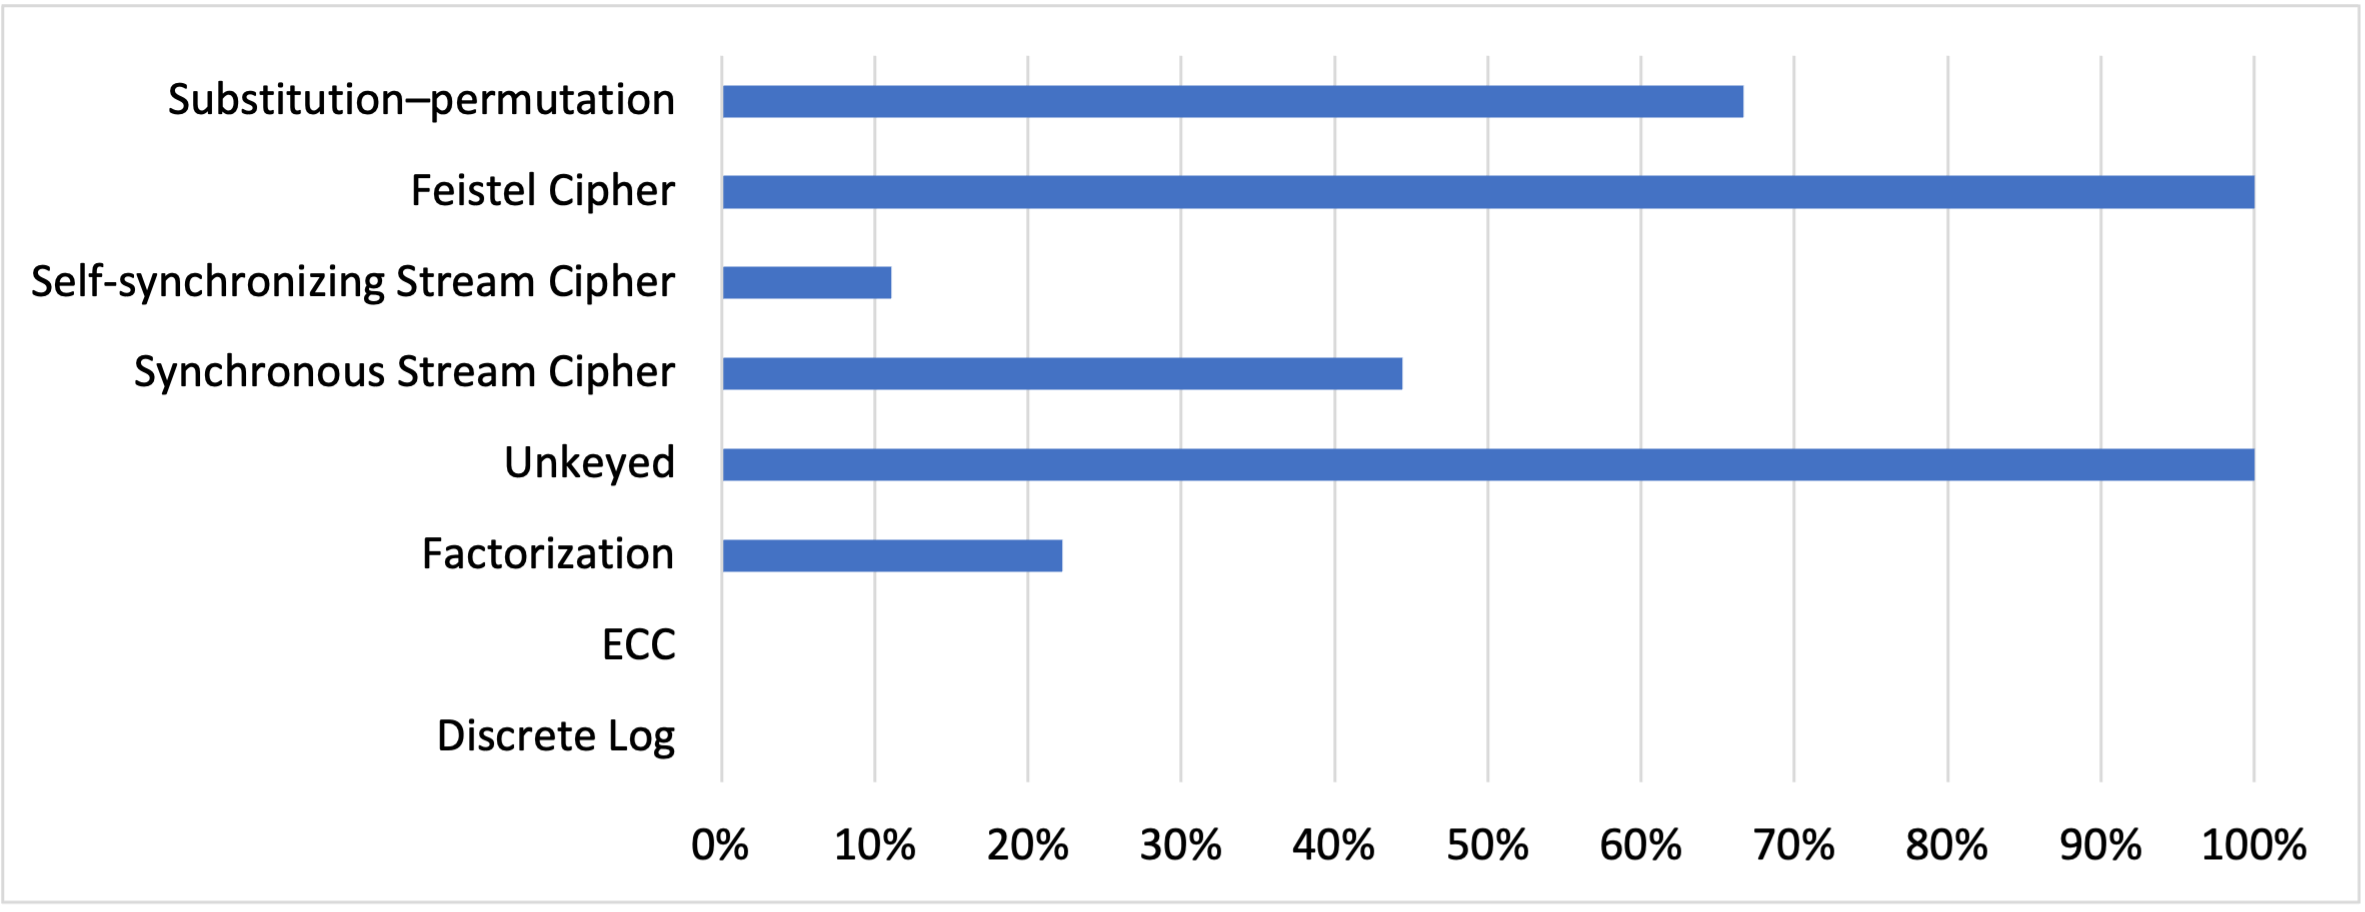
\includegraphics[width=0.95\textwidth]{ch-cryptobinary/figure/algo_percentage.png}
		\caption{Types of cryptographic functionality and designs targeted by different tools and approaches, by percentage of tools surveyed}
		\label{fig:cryptobinary-percentage}
\end{figure}

% \fanyo{To gain a comprehensive understanding of the current state of cryptographic function detection techniques and related tools, we conducted a comprehensive investigation experiment. We introduced numerous new evaluation benchmarks and frameworks that previous research in this field has not explored. Our benchmark will be detailed in Section \ref{sec:framework}, while the experiment results will be presented in Section \ref{sec:evaluation}. Additionally, we will provide discussion based on our evaluation results in Section \ref{sec:discussion}.}




% \fanyo{To gain a comprehensive understanding of the current state of cryptographic function detection techniques and related tools, we conducted a comprehensive investigation experiment. We introduced numerous new evaluation benchmarks and frameworks that previous research in this field has not explored. Our benchmark will be detailed in Section \ref{sec:framework}, while the experiment results will be presented in Section \ref{sec:evaluation}. Additionally, we will provide discussion based on our evaluation results in Section \ref{sec:discussion}.}






% %%%%%%%%%%%%%%%%%%%%%%%%%%%%%%%%%
% \subsection{Research Questions}
% %%%%%%%%%%%%%%%%%%%%%%%%%%%%%%%%%

% We also work to understand how well state-of-the-art techniques and tools perform by proposing and answering the following research questions.  We also believe many of these research questions are still yet unanswered in a satisfactory way, as we discuss more in Section~\ref{sec:evaluation} where we present a number of open research problems in these directions.

% \begin{itemize}
%   \item \textbf{R1} Does the choice of compiler play a role in the detection success? 
%   \item \textbf{R2} Is there any impact from optimization flags?
%   \item \textbf{R3} Are some algorithms easier to detect compared to others? 
%   \item \textbf{R4} Can the same tool perform similarly well across different algorithms?
%   \item \textbf{R5} Is the version of the algorithm significant during detection? 
%   \item \textbf{R6} Are ``malicious'' versions of cryptographic algorithms trickier to detect?

% \end{itemize}




\subsection{Categorization of Cryptographic Algorithm Detection Tools}
\label{subsec:cryptobinary-tool_cat}

We employ a systematic approach to categorize, classify, and interrelate the diverse array of knowledge elements that constitute such cryptographic detection tools from several directions. \autoref{tab:cryptobinary-taxonomy1} contains an overview and summary of each tool, including its reproduction and replication status in this work, as well as a variety of information such that one can easily find or organize existing (and future) tools based on the per-column categories.

We begin by categorizing the detection approach (broken down by the different methods discussed previously in ~\autoref{sec:cryptobinary-detection}) and the programming language in which the tool's source code is written. We note that some tools are not open source; they provide only an executable file, and as a result, we lack information about the source language.
Some tools require specific dependent libraries to run, which can limit or hinder their usability, and as such we list if there are any required dependencies.
Some tools are installation-free and do not require compilation, offering an easy, user-friendly experience.
And a few tools provide the capability for developers to insert new cryptographic algorithm signatures, thereby expanding their detection capabilities as the field advances.
 
\begin{sidewaystable}[p]
\centering
\footnotesize
\renewcommand{\arraystretch}{1.75}

\begin{adjustbox}{max width=0.9\textheight}
\begin{tabular}{c||c|c|c|c|c|c|c|c}
\hline
Tool & Method & \begin{tabular}{@{}c@{}}Dependent\\[-6pt]Library\end{tabular} & Language & \begin{tabular}{@{}c@{}}Requires\\[-6pt]Compiling\end{tabular} & Expandable & R+R & \begin{tabular}{@{}c@{}}Obf. Binary\\[-6pt]Design\end{tabular} & \begin{tabular}{@{}c@{}}AI/ML\\[-6pt]Approach\end{tabular} \\ \hline
\hline
Aligot         & I/O Parameters             & Intel Pin          & Python     & Yes     & Yes     & Reproducible & No  & No  \\ \hline
CryptoHunt     & Bit-precise Symbolic Loop  & Intel Pin          & C++        & Yes     & Yes     & Unable       & Yes & No  \\ \hline
CryptoKnight   & Machine Learning Based     & Intel Pin, PyTorch & Python     & Yes     & Yes     & Both         & No  & Yes \\ \hline
DRACA          & Unknown                    & None               & Executable & No      & No      & Replicable   & No  & No  \\ \hline
FindCrypt2     & Magic Constants            & IDA Pro            & C++        & Yes     & No      & Replicable   & No  & No  \\ \hline
FALKE-MC       & Neural Network             & None               & Unknown    & Unknown & Unknown & Unable       & Yes & Yes \\ \hline
HCD            & Unknown                    & None               & Executable & No      & No      & Replicable   & No  & No  \\ \hline
Kerckhoff      & Multiple                   & Intel Pin          & Python     & No      & Yes     & Unable       & No  & No  \\ \hline
PEiD KANAL     & Signature Searching        & None               & Executable & No      & Yes     & Replicable   & No  & No  \\ \hline
Signsrch       & Signature Searching        & None               & Executable & No      & No      & Replicable   & No  & No  \\ \hline
Softmax Classifier & Neural Network         & Unknown            & Python     & Unknown & Unknown & Unable       & No  & Yes \\ \hline
Where's Crypto & DFG Isomorphism            & IDA SDK            & C++        & Yes     & Yes     & Both         & No  & No  \\ \hline
\end{tabular}
\end{adjustbox}

\caption{Categorization of existing tools and their important properties}
\label{tab:cryptobinary-taxonomy1}
\end{sidewaystable}